\subsubsection{Vectorization}
One of the main reasons for this project was to increase the efficiency of our sponsor's work flow. We realized that ACI was one of the most intensive indices to run so it made sense to look at it first. That being said, one of the biggest problems with the original code is its use of for loops. R is notoriously slow at looping with the only solution being to vectorize the functions you write. To do this we took algorithms being run inside of a for loop and made them in to seperate functions. Once sectioned off these functions could be appropriated to take in vectors and output vectors. This also involved adjusting some of the code after functions to work strictly with vectors. This led to a speed up close to 60\% on an 18 second sound file.

\begin{figure}
	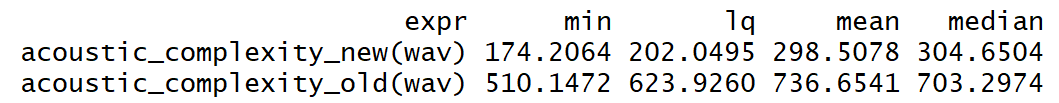
\includegraphics{ACIBenchmark}
\end{figure}

\subsubsection{Memory Challenges}
One of the major challenges that we encountered with the processing of sound files was the massive amounts of RAM needed. We identified the problem to be a third party function called "spectro". Out of the 152MB used to process the 18 second sound file 146MB was used by two instances of "spectro".\par
The first approach was to look for alternatives, but the basic functionality of spectro made it so that all substitutes also used massive amounts of memories. Once we dived into how spectro worked we realized that it was used to make a matrix that represented the intensity of the sound file at every frequency over time. By its very nature the function was going to need a large amount of memory.\par
The second solution was to split the files on the window length and run spectro on smaller chunks. This would increase the run-time of the analysis slightly but reduced the RAM used on an hour long file from 9GB to just under 2GB. The issue with this is that slicing the sound file produced slightly different numbers than the original function. Once we looked into the reason it was found that slicing the files made it so that the spectro function took its measurements at different points. We decided that this would be a problem better solved by someone who had a deeper understanding of the mathematics behind the ACI index.\par
Our final solution was to just limit one job at a time for our application and to require a minimum number of Gig's in order to run our program. While this solution was less than desired we believe that this is something that is not crucial to the product working. That being said this would be an excellent point of improvement for future groups who may be more focused on the research side of this application.\par
\subsubsection{Minor Improvements}
Some small changes were made in order to try and improve the memory usage of the ACI index algorithm. The matrix of intensity changes, used to calculate ACI values, was replaced with on-going calculations. An option was added to include the matrix if desired. With the matrix disabled the memory cost for storing the output decreased from 80KB to 15KB. This improvement is expected to drastically help reduce the size of our database storage needs.